\section{Discussion}

\subsection{Comparison of the spectra at different latitudes}

\begin{figure*}
\vspace*{-0.2cm}
	\makebox[\linewidth][c]{%
	\vspace*{-0.2cm}
		\begin{subfigure}[b]{.4\textwidth}
		\centering 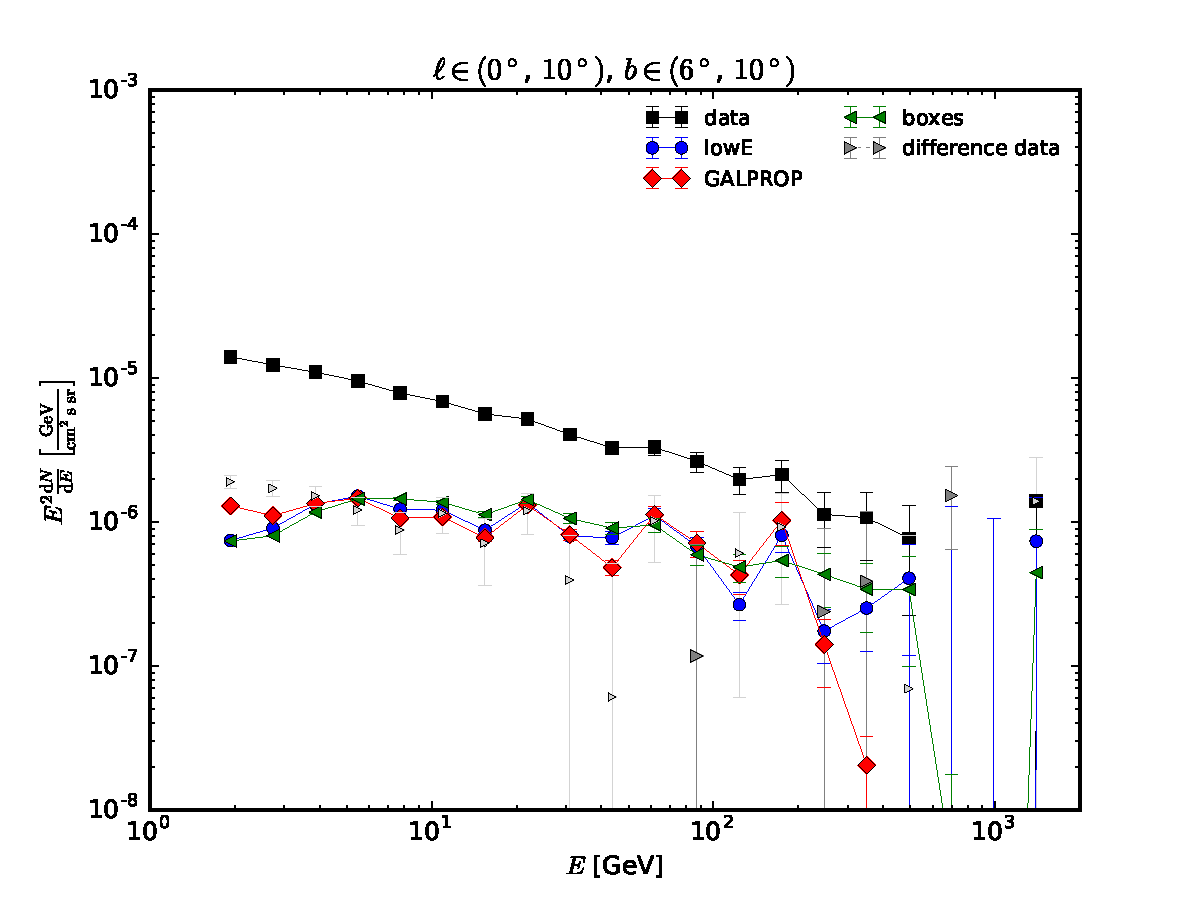
\includegraphics[width=.95\textwidth]{plots/SED_all_left-right__l=5_b=8.pdf}
		\vspace*{-0.2cm}
		\end{subfigure}%
		\begin{subfigure}[b]{.4\textwidth}
		\centering 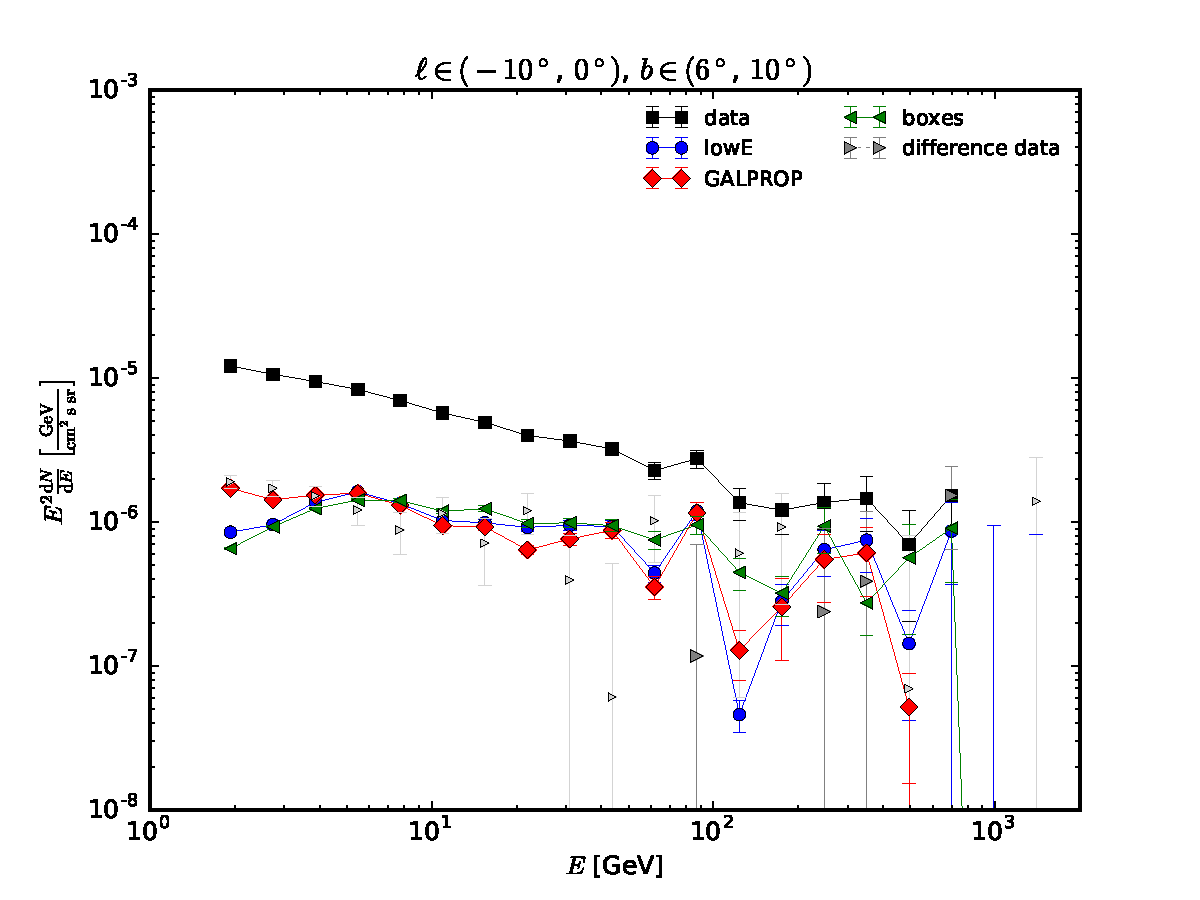
\includegraphics[width=.95\textwidth]{plots/SED_all_left-right__l=-5_b=8.pdf}
		\vspace*{-0.2cm}
	\end{subfigure}%
	\vspace*{-0.2cm}
	}\\
	\vspace*{-0.2cm}
	\makebox[\linewidth][c]{%
		\begin{subfigure}[b]{.4\textwidth}
		\centering 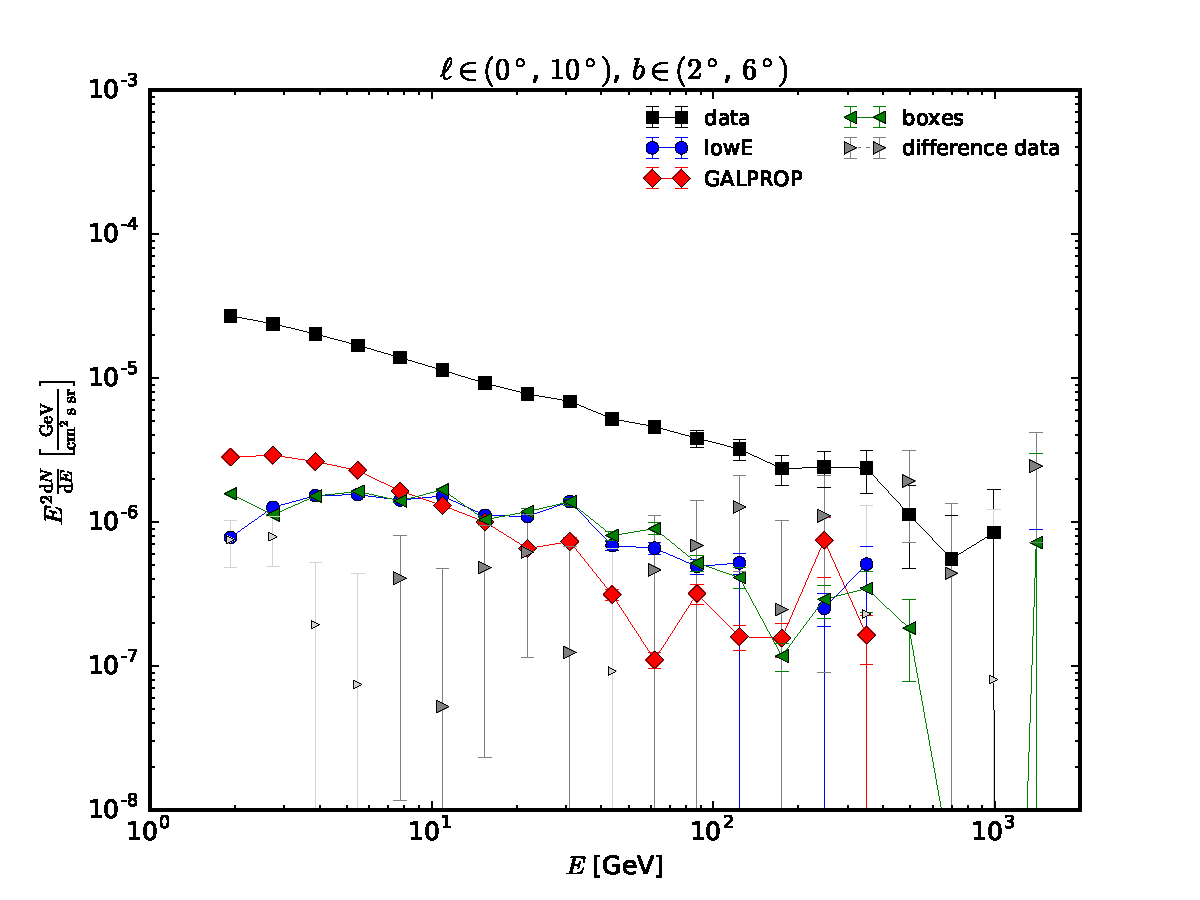
\includegraphics[width=.95\textwidth]{plots/SED_all_left-right__l=5_b=4.pdf}
		\end{subfigure}%
		\begin{subfigure}[b]{.4\textwidth}
		\centering 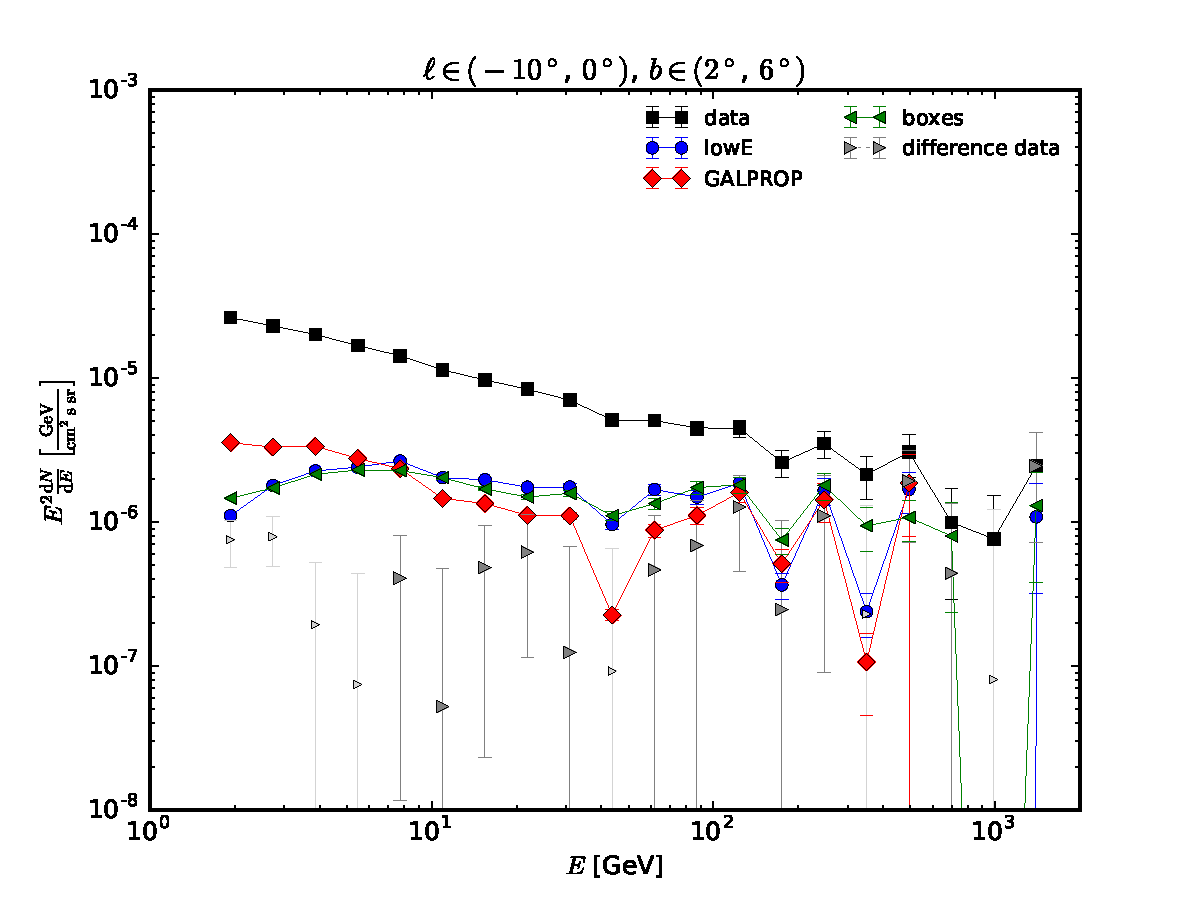
\includegraphics[width=.95\textwidth]{plots/SED_all_left-right__l=-5_b=4.pdf}
	\end{subfigure}%
}
\vspace*{-0.2cm}
	\makebox[\linewidth][c]{%
		\begin{subfigure}[b]{.4\textwidth}
		\centering 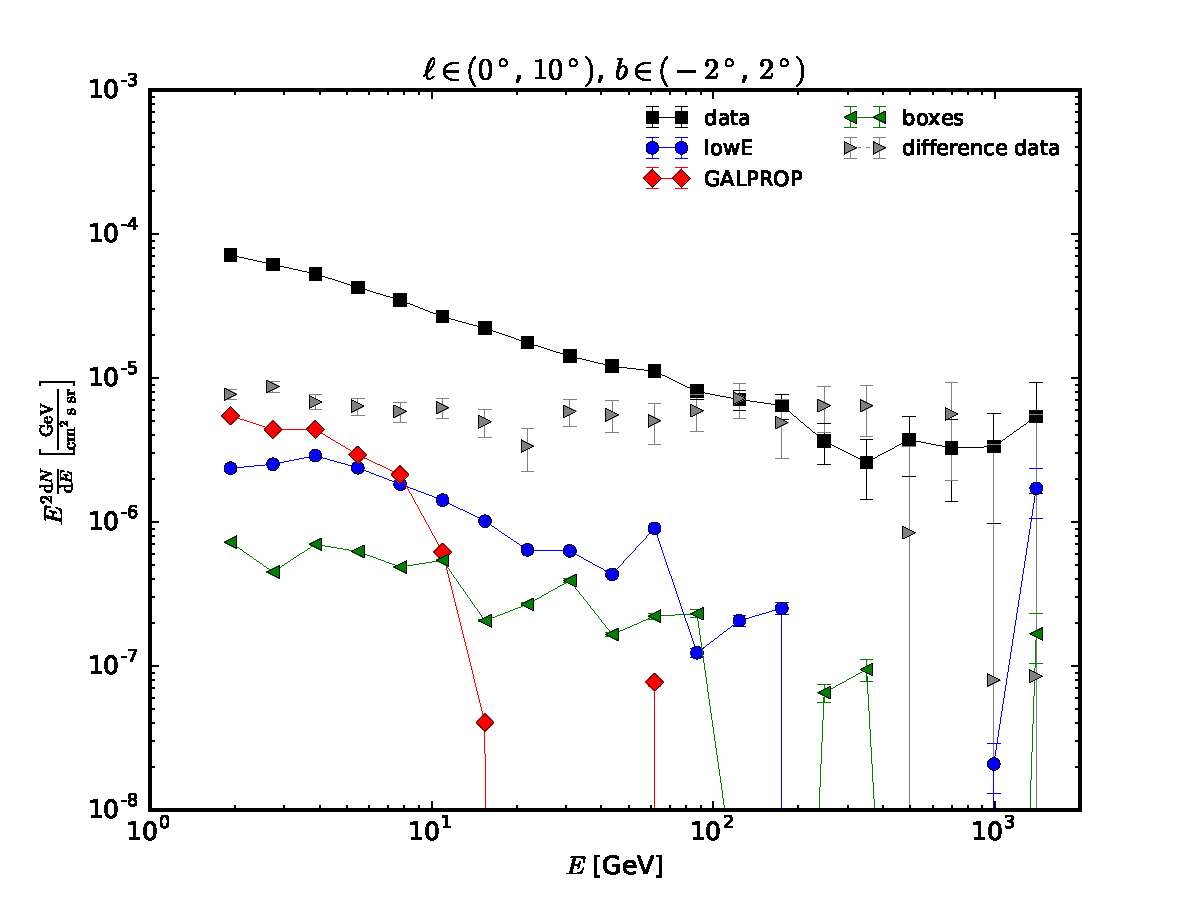
\includegraphics[width=.95\textwidth]{plots/SED_all_left-right__l=5_b=0.pdf}
		\end{subfigure}%
		\begin{subfigure}[b]{.4\textwidth}
		\centering 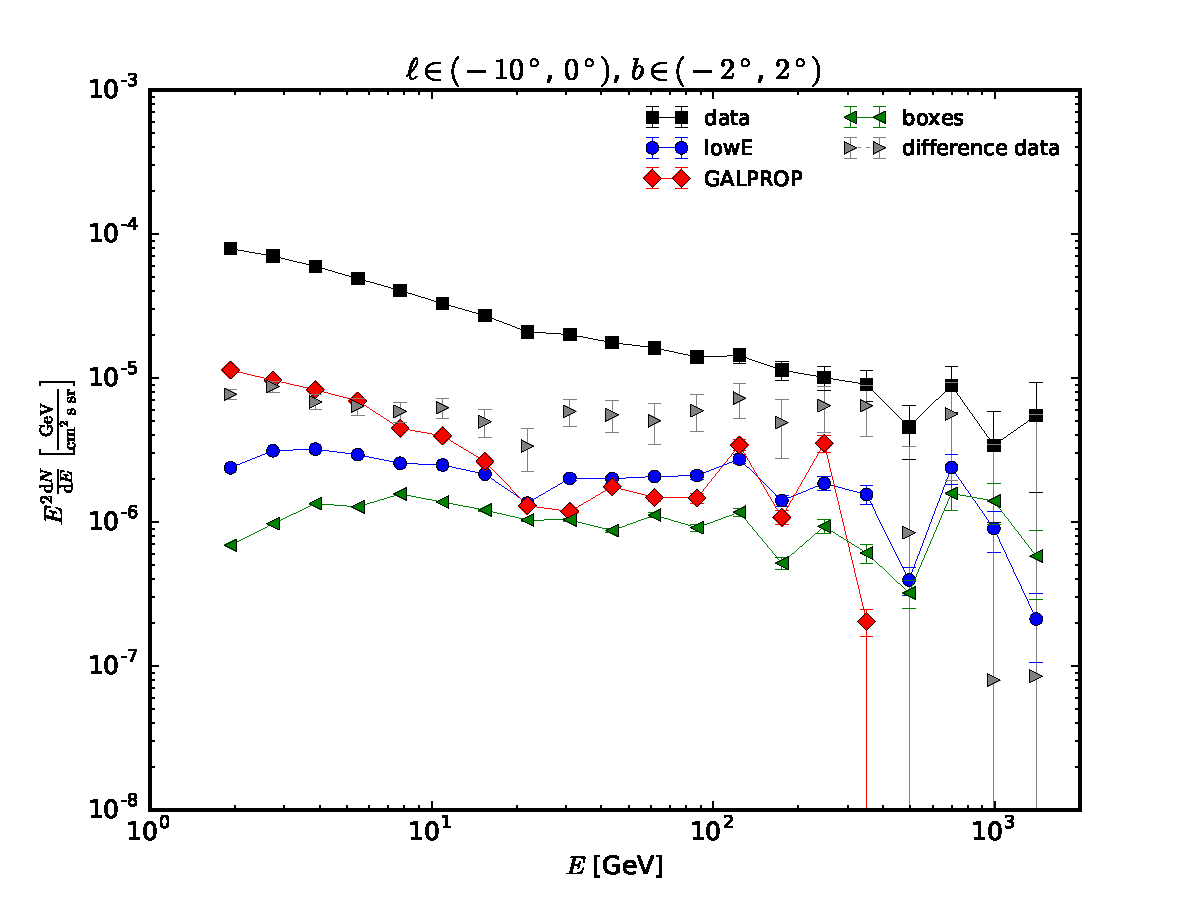
\includegraphics[width=.95\textwidth]{plots/SED_all_left-right__l=-5_b=0.pdf}
	\end{subfigure}%
}
\vspace*{-0.2cm}
	\makebox[\linewidth][c]{%
		\begin{subfigure}[b]{.4\textwidth}
		\centering 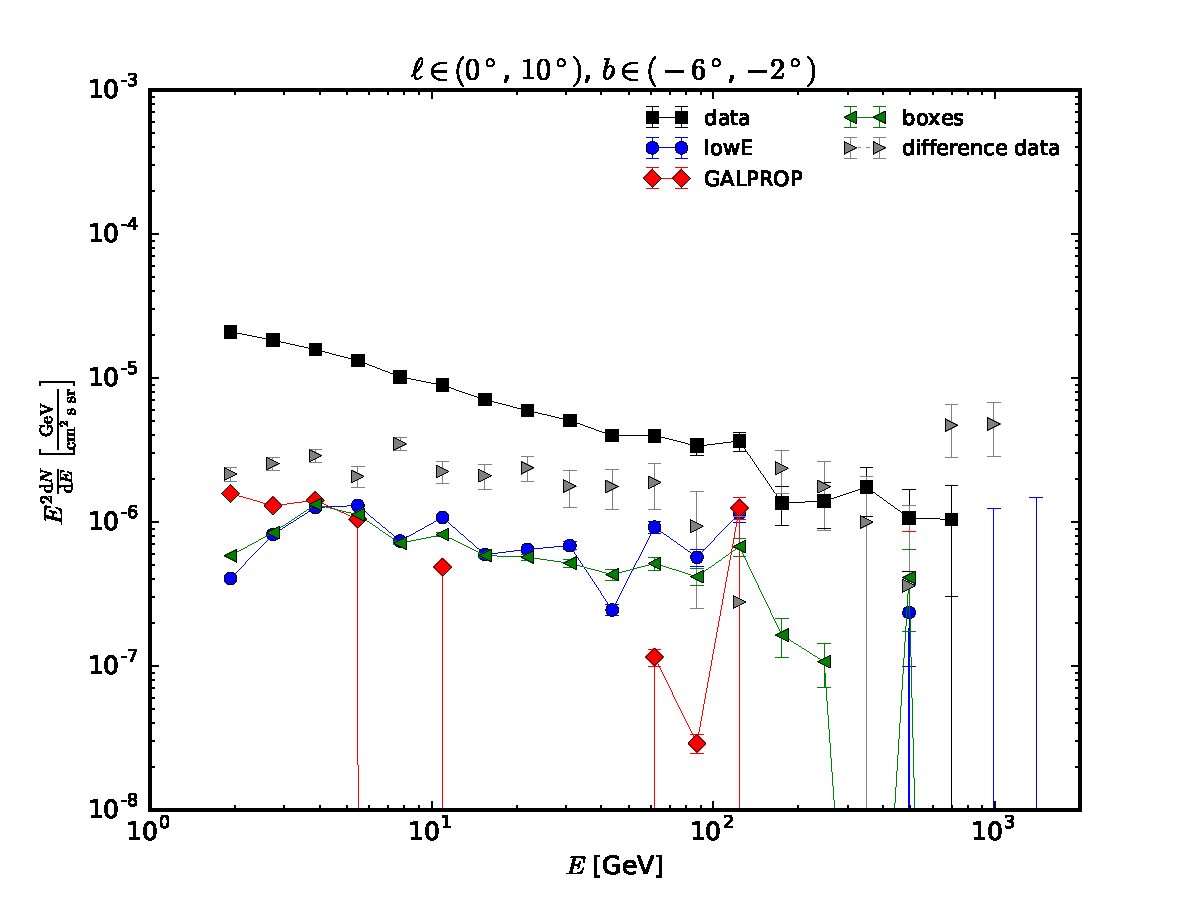
\includegraphics[width=.95\textwidth]{plots/SED_all_left-right__l=5_b=-4.pdf}
		\end{subfigure}%
		\begin{subfigure}[b]{.4\textwidth}
		\centering 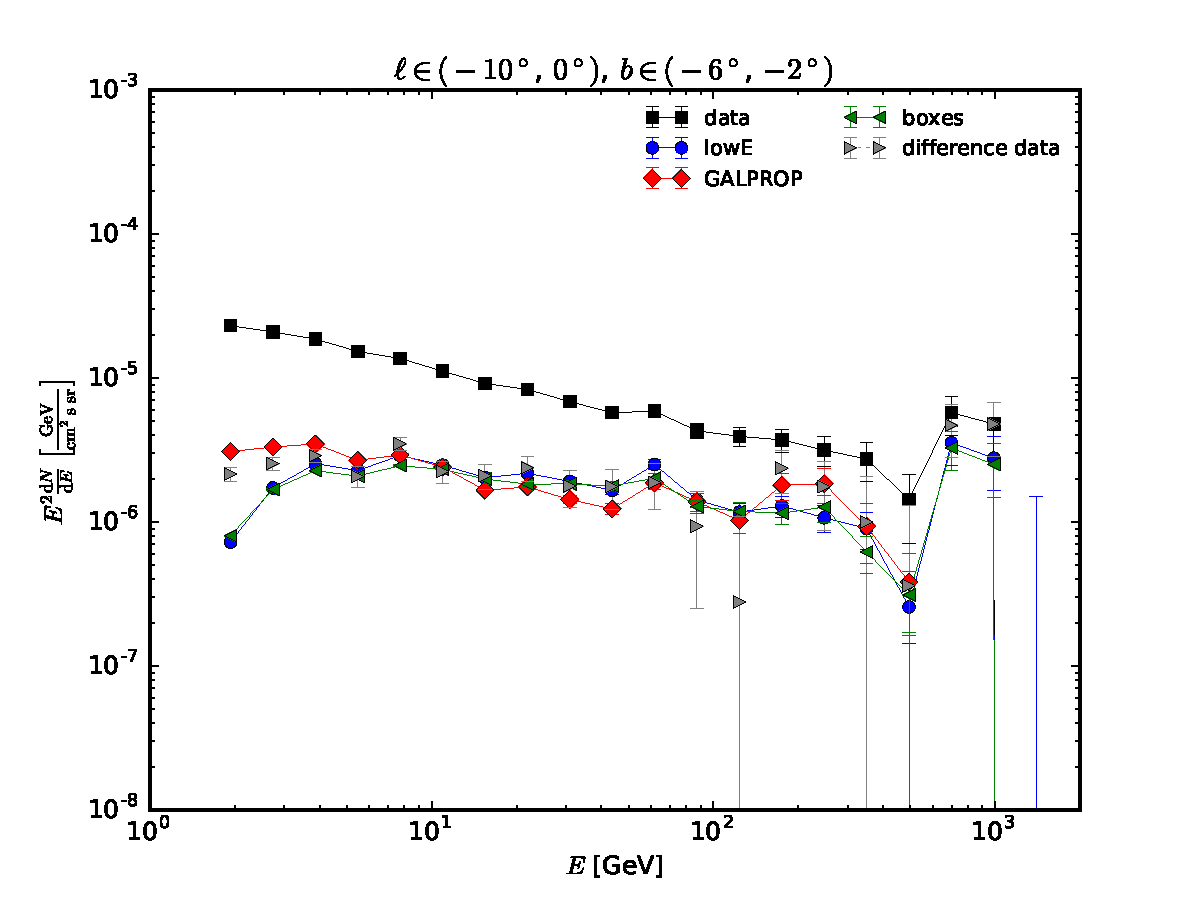
\includegraphics[width=.95\textwidth]{plots/SED_all_left-right__l=-5_b=-4.pdf}
	\end{subfigure}%
}
\vspace*{-0.2cm}
	\makebox[\linewidth][c]{%
		\begin{subfigure}[b]{.4\textwidth}
		\centering 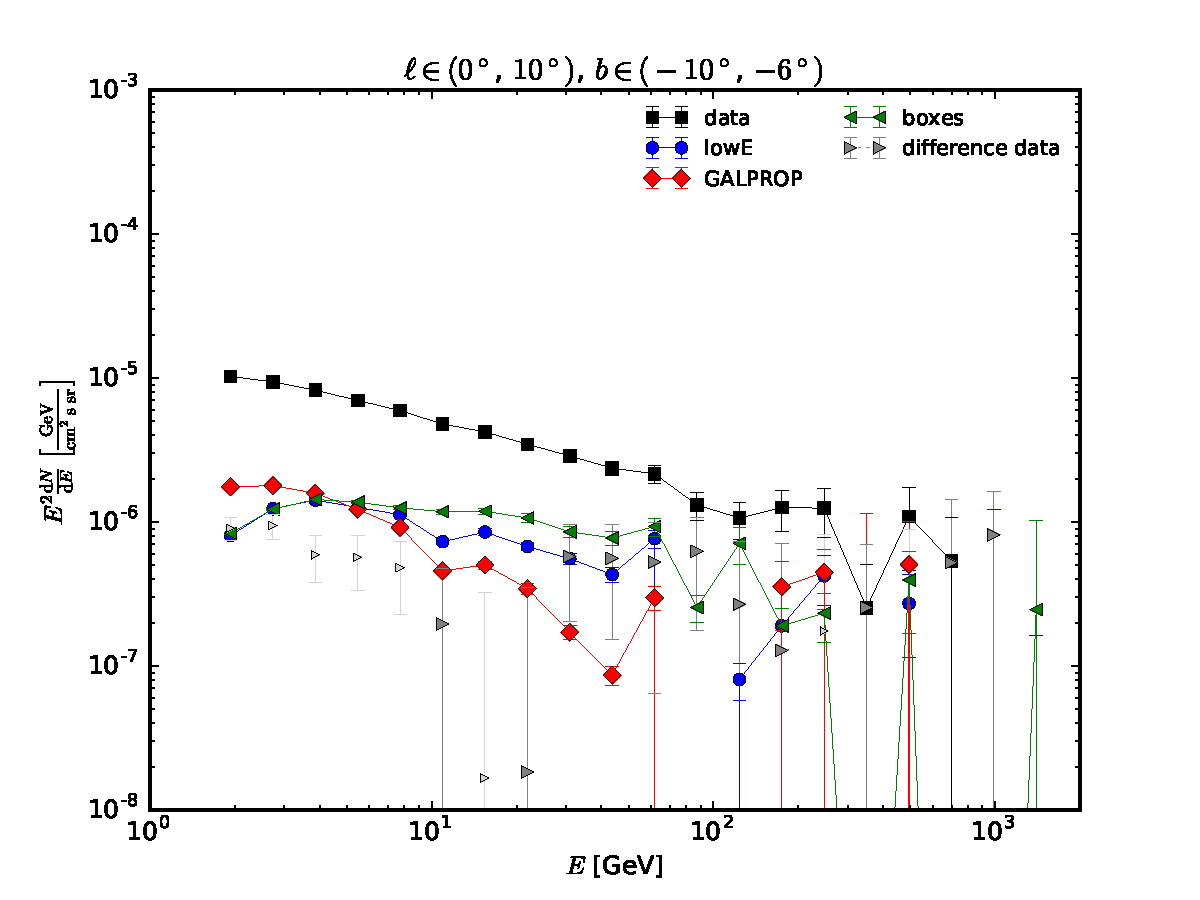
\includegraphics[width=.95\textwidth]{plots/SED_all_left-right__l=5_b=-8.pdf}
		\end{subfigure}%
		\begin{subfigure}[b]{.4\textwidth}
		\centering 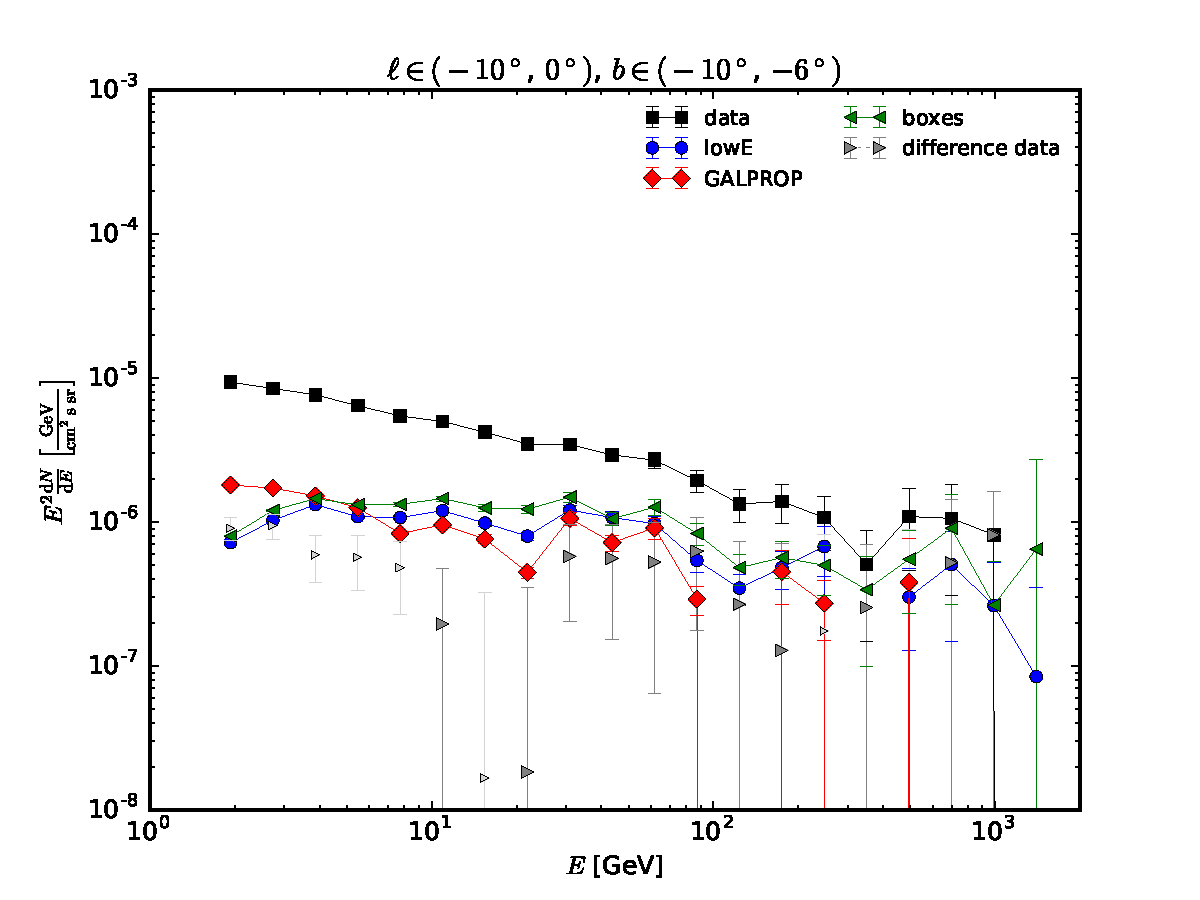
\includegraphics[width=.95\textwidth]{plots/SED_all_left-right__l=-5_b=-8.pdf}
	\end{subfigure}%
}
\caption{Spectra.}
\label{Spectra_all}
\end{figure*}



\subsection{Profile plots}

Figure \ref{Profiles_all} shows the latitude profiles of the different models in differential flux. The flux increases towards the Galactic plane. Left-right assymmetry close to the Galactic center. 


\begin{figure*}[h!]
    \begin{subfigure}{0.5\textwidth}
        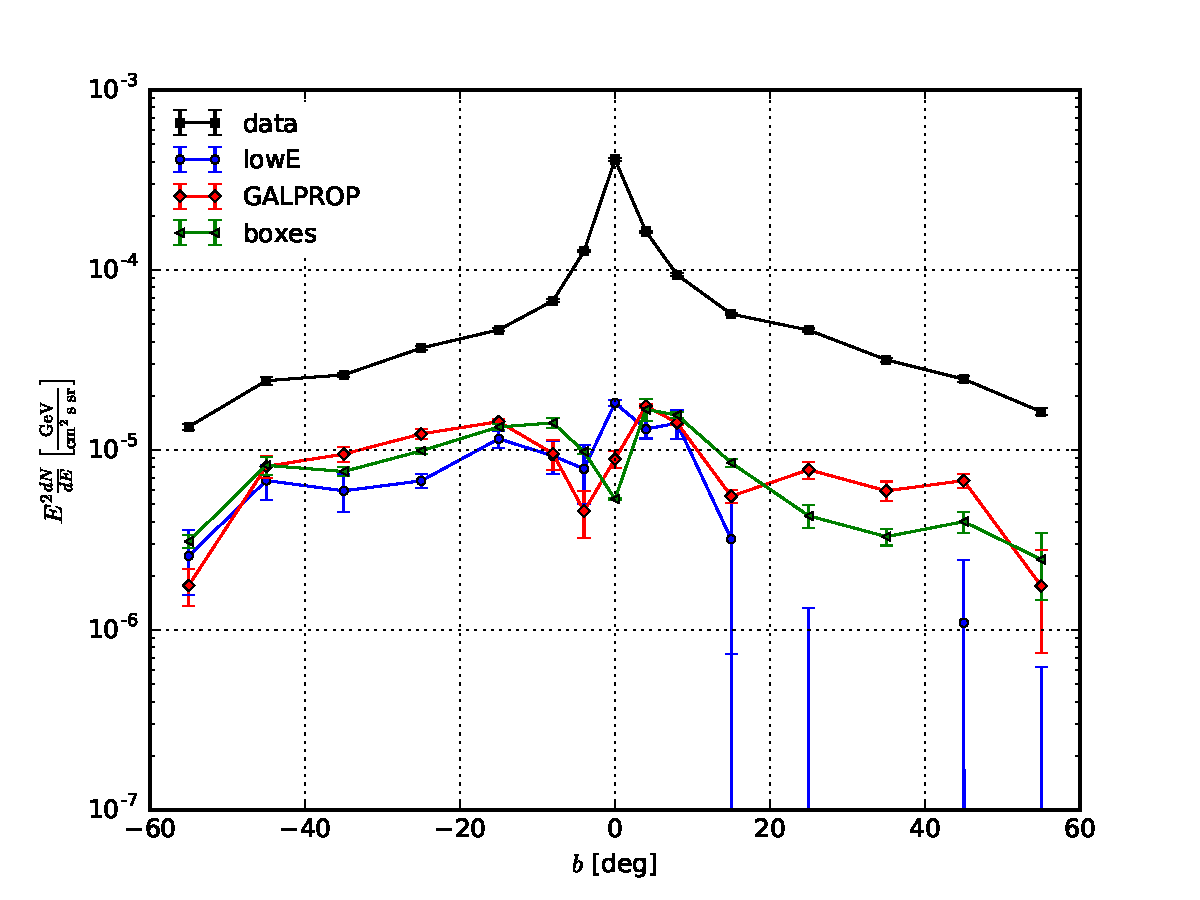
\includegraphics[width=\textwidth]{plots/Profiles_left.pdf}
    \end{subfigure} 
    \begin{subfigure}{0.5\textwidth}
        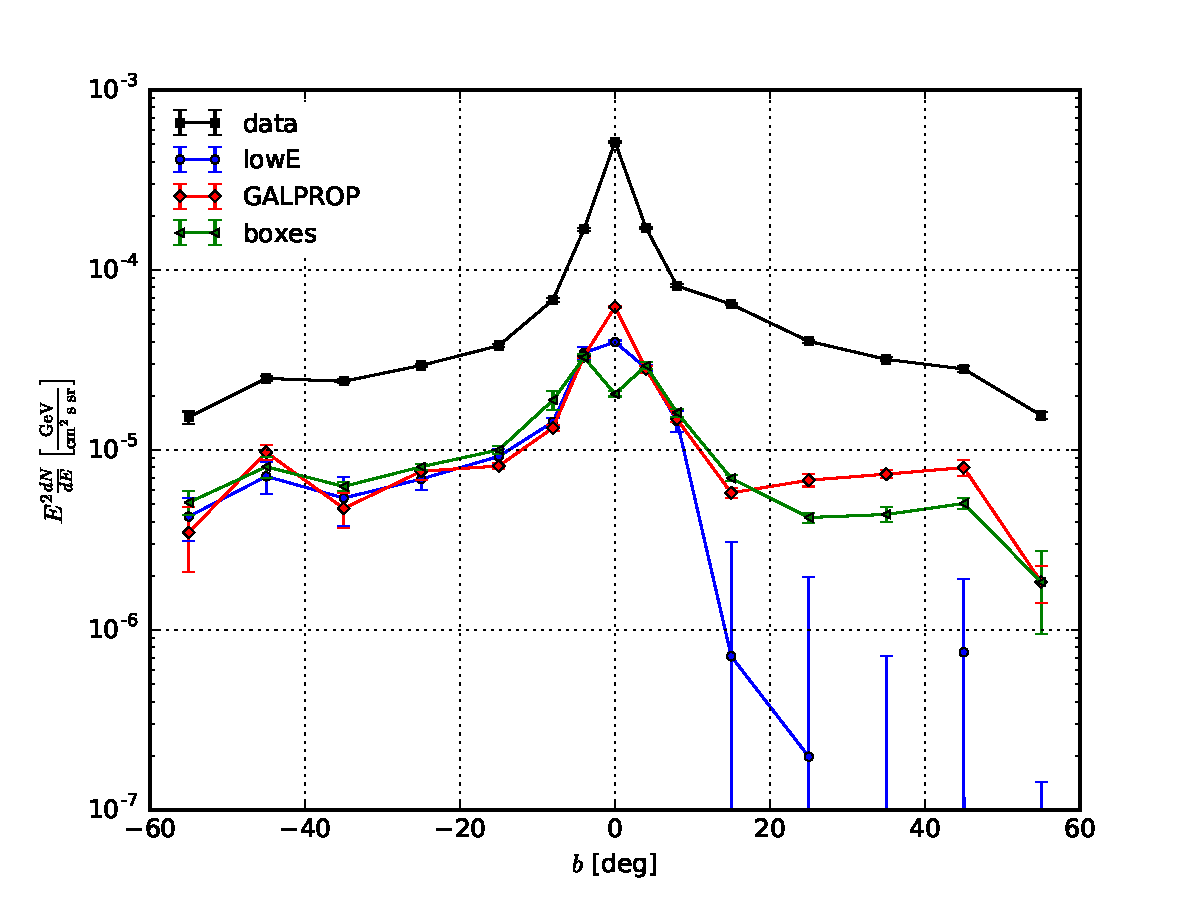
\includegraphics[width=\textwidth]{plots/Profiles_right.pdf}
    \end{subfigure}
  	\caption{Latitude profiles of the different models.}
  	\label{Profiles_all}
\end{figure*}

\subsection{IC model}


\subsection{Pion model}